\documentclass{article}

\usepackage{hyperref}  % Clickable links in PDFs.
\usepackage{setspace}
\usepackage[separate-uncertainty,multi-part-units=single]{siunitx}  % Units
\usepackage{amsmath}
\usepackage[margin=1.5in]{geometry}  % Document margins.
\usepackage{graphicx}  % Figures.
\usepackage{subcaption}  % Subfigures.
\usepackage{cleveref}  % Use \cref{} instead of \ref{}
\usepackage{glossaries}
\usepackage{todonotes}  % Use \todo{Not done yet.} for margin notes.

% Resize figures to fit by default.
\setkeys{Gin}{width=\textwidth,keepaspectratio}

% Acronyms etc.
\loadglsentries{glossary}
\makeglossaries

% Formatting for supplementals.
\newcommand{\beginsupplement}{
    \setcounter{table}{0}
    \renewcommand{\thetable}{S\arabic{table}}
    \setcounter{figure}{0}
    \renewcommand{\thefigure}{S\arabic{figure}}
}

\title{My Awesome Document}
\author{Emerson Harkin}

\begin{document}

\maketitle
\newpage

\tableofcontents
\listoffigures
\printglossaries

\newpage

\doublespacing

\section{Introduction}
\subsection{Cleverref} \label{sec:intro_part}

This section demonstrates why cleverref is useful.

\begin{table}
    \caption{A table.}
    \begin{tabular}{ccc}
        Column & Column & Column \\ \hline
        One & Two & Three
    \end{tabular}
    \label{tab:exampletable}
\end{table}

\begin{align}
    E &= mc^2 \label{eqn:einstein} \\
    \frac{dz}{dt} &= \frac{z_\infty - z}{\tau} \label{eqn:nonsense}
\end{align}

Using cleverref we can refer to \cref{eqn:einstein}, \cref{sec:intro_part}, and
\cref{tab:exampletable} with a simple call to \verb|\cref{}| and let cleverref
figure out whether the environment being referenced is a section, table, etc.

\subsection{Acronyms}

\LaTeX glossaries automatically print the long-form version of an acronym the
first time it is used. Here's an example.

The \gls{drn} and \gls{mpfc} are brain regions with neurons. The \gls{drn}
is made up mainly of \gls{ser} cells. \Gls{som} neurons are found in both the
\gls{mpfc} and \gls{drn}.


\section{Results}
\subsection{Figures}

Results often have figures, but in this case \cref{fig:real_fig} is the only
real figure. There may also be supplementary figures (e.g.,
\cref{fig:supplemental}).

\begin{figure}
    \begin{subfigure}{0.22\textwidth}
        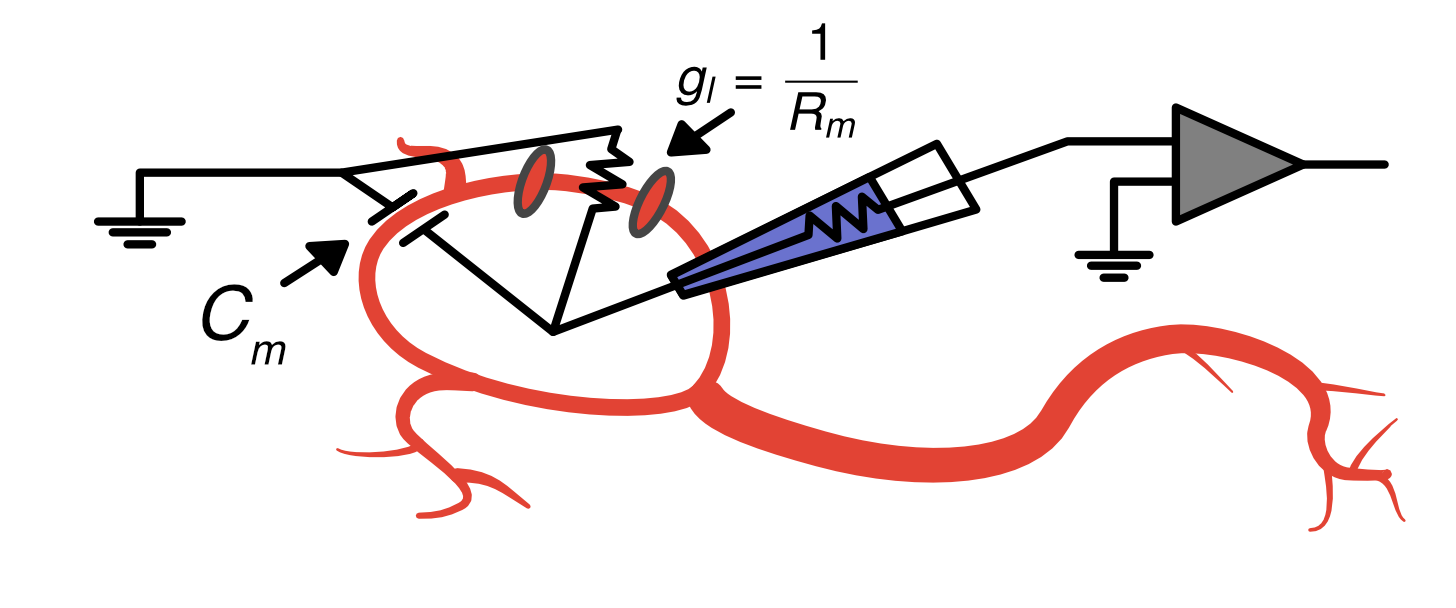
\includegraphics{img/GIF_circuit.png}
        \caption{Useful caption.}
        \label{fig:real_fig}
    \end{subfigure}
    \begin{subfigure}{0.22\textwidth}
        \includegraphics{example-image}
        \caption{Another caption.}
    \end{subfigure}
    \begin{subfigure}{0.3\textwidth}
        \includegraphics[height=1in]{example-image}
        \caption{One more caption.}
    \end{subfigure}
    \caption{Main figure caption.}
\end{figure}



\newpage
\appendix
\beginsupplement
\begin{figure}[h!]
    \includegraphics{example-image}
    \caption{A supplementary figure.}
    \label{fig:supplemental}
\end{figure}


\end{document}
